% mainfile: ../../../main.tex
\chapter{Additional measurements}\label{ch:app:exp:observations}

\begin{margintable}
    \centering
    \footnotesize
    \caption{
        Heterostructure parameters used in \thethesis.
        The doping density $N_{\mr{d}}$ is nominal, whereas the charge carrier density in the \gls{qw}, $n$, is computed using the nominal doping values with parameters given in \cref{tab:app:exp:samples:ps}.
    }
    \label{tab:app:exp:samples}
    \begin{tabularx}{\marginparwidth}{@{} l @{} S[table-alignment=right, table-format=1.1e1] S[table-alignment=right, table-format=1.2e2] @{}}
        \toprule
        \textsc{Wafer}  & {$N_{\mr{d}}$ (\unit{\per\cubic\centi\meter})} & {$n$ (\unit{\per\square\centi\meter})} \\
        \midrule
        M1\_05\_49      & 6.5e17                                         & 1.95e11 \\
        15460 (Honey)   & 1.8e18                                         & 4.26e11 \\
        15271 (Fig)     & 8.0e17                                         & 3.91e11 \\
        \bottomrule
    \end{tabularx}
\end{margintable}

\begin{margintable}
    \centering
    \footnotesize
    \begin{threeparttable}
        \caption{
            Simulation parameters used to compute the charge carrier density $n$ in \cref{tab:app:exp:samples}.
            $E_{\mr{DX}}$ is the
        }
        \label{tab:app:exp:samples:ps}
        \begin{tabularx}{2cm}{c c}
            \toprule
            $E_{\mr{DX}}$\tnote{a}          & \qty{-71.5}{meV} \\
            $\Delta E_{\mr{c}}$\tnote{b}    & \qty{240}{meV} \\
            $m_{\mr{c}}$                    & \num{0.067}{$m_e$} \\
            $\Delta z$                      & \qty{0.5}{nm} \\
            $T$                             & \qty{10}{mK} \\
            $V_{\mr{FP}}$\tnote{c}          & \qty{0.76}{V} \\
            \bottomrule
        \end{tabularx}
        \begin{tablenotes}
            \scriptsize
            \item[a] Energy of the DX-center below the Fermi level.
            \item[b] Conduction band offset at the \ch{GaAs/AlGaAs} interface.
            \item[c] Fermi level pinning voltage.
        \end{tablenotes}
    \end{threeparttable}
\end{margintable}
%

\begin{marginfigure}
    \centering
    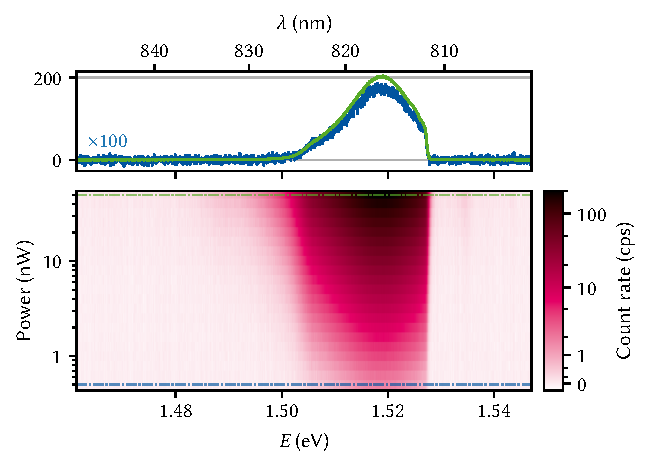
\includegraphics{img/pdf/experiment/2deg_pl_power_dependence}
    \caption[
        \sampleid{Doped M1_05_49-2}
        \thewavelength{795}
        \protect\newline
        \imgsource{img/py/experiment/pl.py}
    ]{}
    \label{fig:app:exp:observations:2deg_pl_power_dependence}
\end{marginfigure}

\begin{figure}
    \centering
    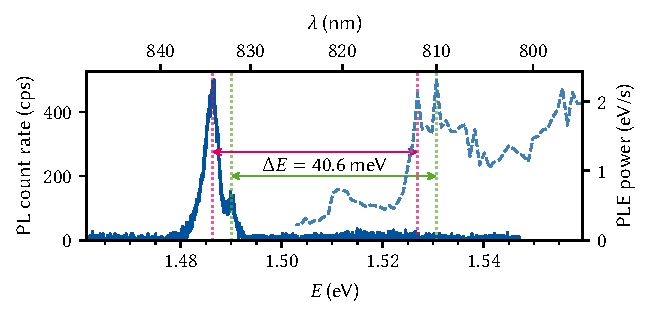
\includegraphics{img/pdf/experiment/doped_M1_05_49-2_ple_single}
    \caption[
        \sampleid{Doped M1_05_49-2}
        \thevoltage{-1.3}{CM}
        \thepower{1}{\micro}
        \protect\newline
        \imgsource{img/py/experiment/ple.py}
    ]{
    }
    \label{fig:app:exp:pl:doped_M1_05_49-2_ple}
\end{figure}
